\documentclass[conference]{IEEEtran}
\IEEEoverridecommandlockouts
% The preceding line is only needed to identify funding in the first footnote. If that is unneeded, please comment it out.
\usepackage{cite}
\usepackage{amsmath,amssymb,amsfonts}
\usepackage{algpseudocode}
\usepackage{algorithm}
\usepackage{graphicx}
\usepackage{textcomp}
\usepackage{xcolor}
\usepackage{multirow}
\def\BibTeX{{\rm B\kern-.05em{\sc i\kern-.025em b}\kern-.08em
    T\kern-.1667em\lower.7ex\hbox{E}\kern-.125emX}}
\begin{document}

\title{SALCA-IB: Self-Adaptive LLM-Driven Continuous Learning Agent for IB Network Failure Prediction\\
{\footnotesize \textsuperscript{*}Note: Sub-titles are not captured in Xplore and
should not be used}
\thanks{Identify applicable funding agency here. If none, delete this.}
}

\author{\IEEEauthorblockN{1\textsuperscript{st} Given Name Surname}
\IEEEauthorblockA{\textit{dept. name of organization (of Aff.)} \\
\textit{name of organization (of Aff.)}\\
City, Country \\
email address or ORCID}
\and
\IEEEauthorblockN{2\textsuperscript{nd} Given Name Surname}
\IEEEauthorblockA{\textit{dept. name of organization (of Aff.)} \\
\textit{name of organization (of Aff.)}\\
City, Country \\
email address or ORCID}
\and
\IEEEauthorblockN{3\textsuperscript{rd} Given Name Surname}
\IEEEauthorblockA{\textit{dept. name of organization (of Aff.)} \\
\textit{name of organization (of Aff.)}\\
City, Country \\
email address or ORCID}
\and
\IEEEauthorblockN{4\textsuperscript{th} Given Name Surname}
\IEEEauthorblockA{\textit{dept. name of organization (of Aff.)} \\
\textit{name of organization (of Aff.)}\\
City, Country \\
email address or ORCID}
\and
\IEEEauthorblockN{5\textsuperscript{th} Given Name Surname}
\IEEEauthorblockA{\textit{dept. name of organization (of Aff.)} \\
\textit{name of organization (of Aff.)}\\
City, Country \\
email address or ORCID}
\and
\IEEEauthorblockN{6\textsuperscript{th} Given Name Surname}
\IEEEauthorblockA{\textit{dept. name of organization (of Aff.)} \\
\textit{name of organization (of Aff.)}\\
City, Country \\
email address or ORCID}
}

\maketitle

\begin{abstract}
The emergence of transformer-based large language models has led to unprecedented demands on high-performance computing infrastructure, where InfiniBand (IB) networks play a vital role for their superior low-latency and high-bandwidth communication capabilities. Network failures in these environments can cause significant training interruptions or restarts, resulting in substantial computational resource waste and training cost overhead. However, effective failure prediction remains challenging due to both the scarcity of failure data and the susceptibility of network features to environmental changes. This paper introduces \textbf{SALCA-IB} (Self-Adaptive LLM-Driven Continuous Learning Agent for IB Network Failure Prediction), an innovative failure prediction system that leverages Large Language Models (LLMs) as its planning core. The system's key innovations include: (1) LLM-driven autonomous data selection and model optimization; (2) A fusion memory system integrating short-term and long-term memory; and (3) LLM-supported automatic evaluation feedback and closed-loop optimization. Experimental results on a production cluster with 2048 computing cards show that SALCA-IB improves prediction F1@K-score by 6.8\% in static scenarios and demonstrates a 15.9\% increase when facing changes in network feature distributions, significantly enhancing the predictability of large-scale computing infrastructure.
\end{abstract}

\begin{IEEEkeywords}
    InfiniBand Network, Large Language Model, Autonomous Agent
\end{IEEEkeywords}

\section{Introduction}
The rapid advancement of transformer-based language models has fundamentally transformed the landscape of artificial intelligence, leading to unprecedented demands on computing infrastructure. Training these increasingly large models, often comprising hundreds of billions of parameters, requires massive distributed computing resources with high-performance interconnects. In such environments, InfiniBand (IB) networks have become the de facto standard for their exceptional performance in low-latency, high-bandwidth communication, serving as the critical backbone for distributed training tasks.

Network failures in distributed training environments can have severe consequences. When IB network failures occur during model training, they often cause unexpected training interruptions or complete restarts, leading to significant computational resource waste and increased operational costs. For instance, recent studies have shown that network-related failures can account for up to 30\% of training interruptions in large-scale AI clusters, with each incident potentially wasting hundreds of GPU hours (He et al. \cite{b6}). This challenge becomes particularly acute as models grow larger and training runs extend to weeks or even months.

Despite its critical importance, effective IB network failure prediction faces several significant challenges. First, failure data in production environments is inherently scarce, as failures are relatively rare events in well-maintained systems, making it difficult to build robust prediction models using traditional machine learning approaches. Second, network feature distributions are highly dynamic and susceptible to various external factors (Liu et al. \cite{b8}), such as environmental conditions, hardware aging, and maintenance activities. These challenges are further compounded by the increasing scale and complexity of modern computing infrastructures.

Traditional approaches to network failure prediction primarily rely on static machine learning models or rule-based systems (Mohammed et al. \cite{b9}, Nie et al. \cite{b10}). While these methods have shown some success in controlled environments, they struggle to maintain performance in real-world scenarios where network characteristics evolve continuously. Moreover, existing solutions often operate as black boxes, providing limited interpretability and failing to leverage historical experience effectively for continuous improvement (Das et al. \cite{b5}). Recent advances in deep learning-based approaches have attempted to address these limitations, but they still face challenges in adapting to dynamic environments and maintaining long-term prediction accuracy (Alharthi et al. \cite{b2}).

The emergence of Large Language Models (LLMs) presents new opportunities for addressing these challenges. LLMs have demonstrated remarkable capabilities in complex reasoning and planning tasks (Ahmed et al. \cite{b1}, Su et al. \cite{b12}), suggesting their potential for orchestrating adaptive prediction systems. Additionally, recent advances in memory systems and continuous learning architectures (Zhang et al. \cite{b13}) have shown promise in handling dynamic environments, though their application to IB network failure prediction remains largely unexplored.

To address these challenges, we propose SALCA-IB (Self-Adaptive LLM-Driven Continuous Learning Agent for IB Network Failure Prediction), an innovative system that combines the reasoning capabilities of LLMs with traditional machine learning models in a unified, adaptive framework. To tackle the data scarcity challenge, SALCA-IB employs an LLM-driven planning core that intelligently orchestrates data selection and model optimization. To handle dynamic feature distributions, we design a dual-memory system that integrates both short-term and long-term experiences. Furthermore, to ensure sustained prediction accuracy, we implement a continuous learning mechanism with LLM-supported feedback loops that enables real-time adaptation to changing network conditions.

The main contributions of this paper are threefold:
\begin{itemize}
    \item We propose an innovative LLM-driven agent architecture for IB network failure prediction that uniquely leverages LLM as a high-level planning core to orchestrate model selection, parameter optimization, and continuous learning strategies, while employing traditional machine learning models as efficient executors for real-time prediction tasks.
    \item We design a novel dual-memory fusion system that seamlessly integrates short-term and long-term memory mechanisms, enabling rapid adaptation to dynamic network changes while preserving and leveraging valuable historical knowledge for enhanced prediction robustness.
    \item We conduct comprehensive experiments on a large-scale production cluster with 2048 computing cards, demonstrating that SALCA-IB improves prediction F1@K-score by 6.8\% under static conditions and achieves a 15.9\% increase when facing network feature distribution changes. Through extensive ablation studies, we validate the substantial contributions of both the LLM-driven framework and the dual-memory system components.
\end{itemize}

The remainder of this paper is organized as follows: Section II reviews related work in HPC failure prediction and LLM applications. Section III details the design and implementation of SALCA-IB. Section IV presents our experimental setup and results. Finally, Section V concludes the paper and discusses future work.

\begin{figure*}[htbp]
    \centering
    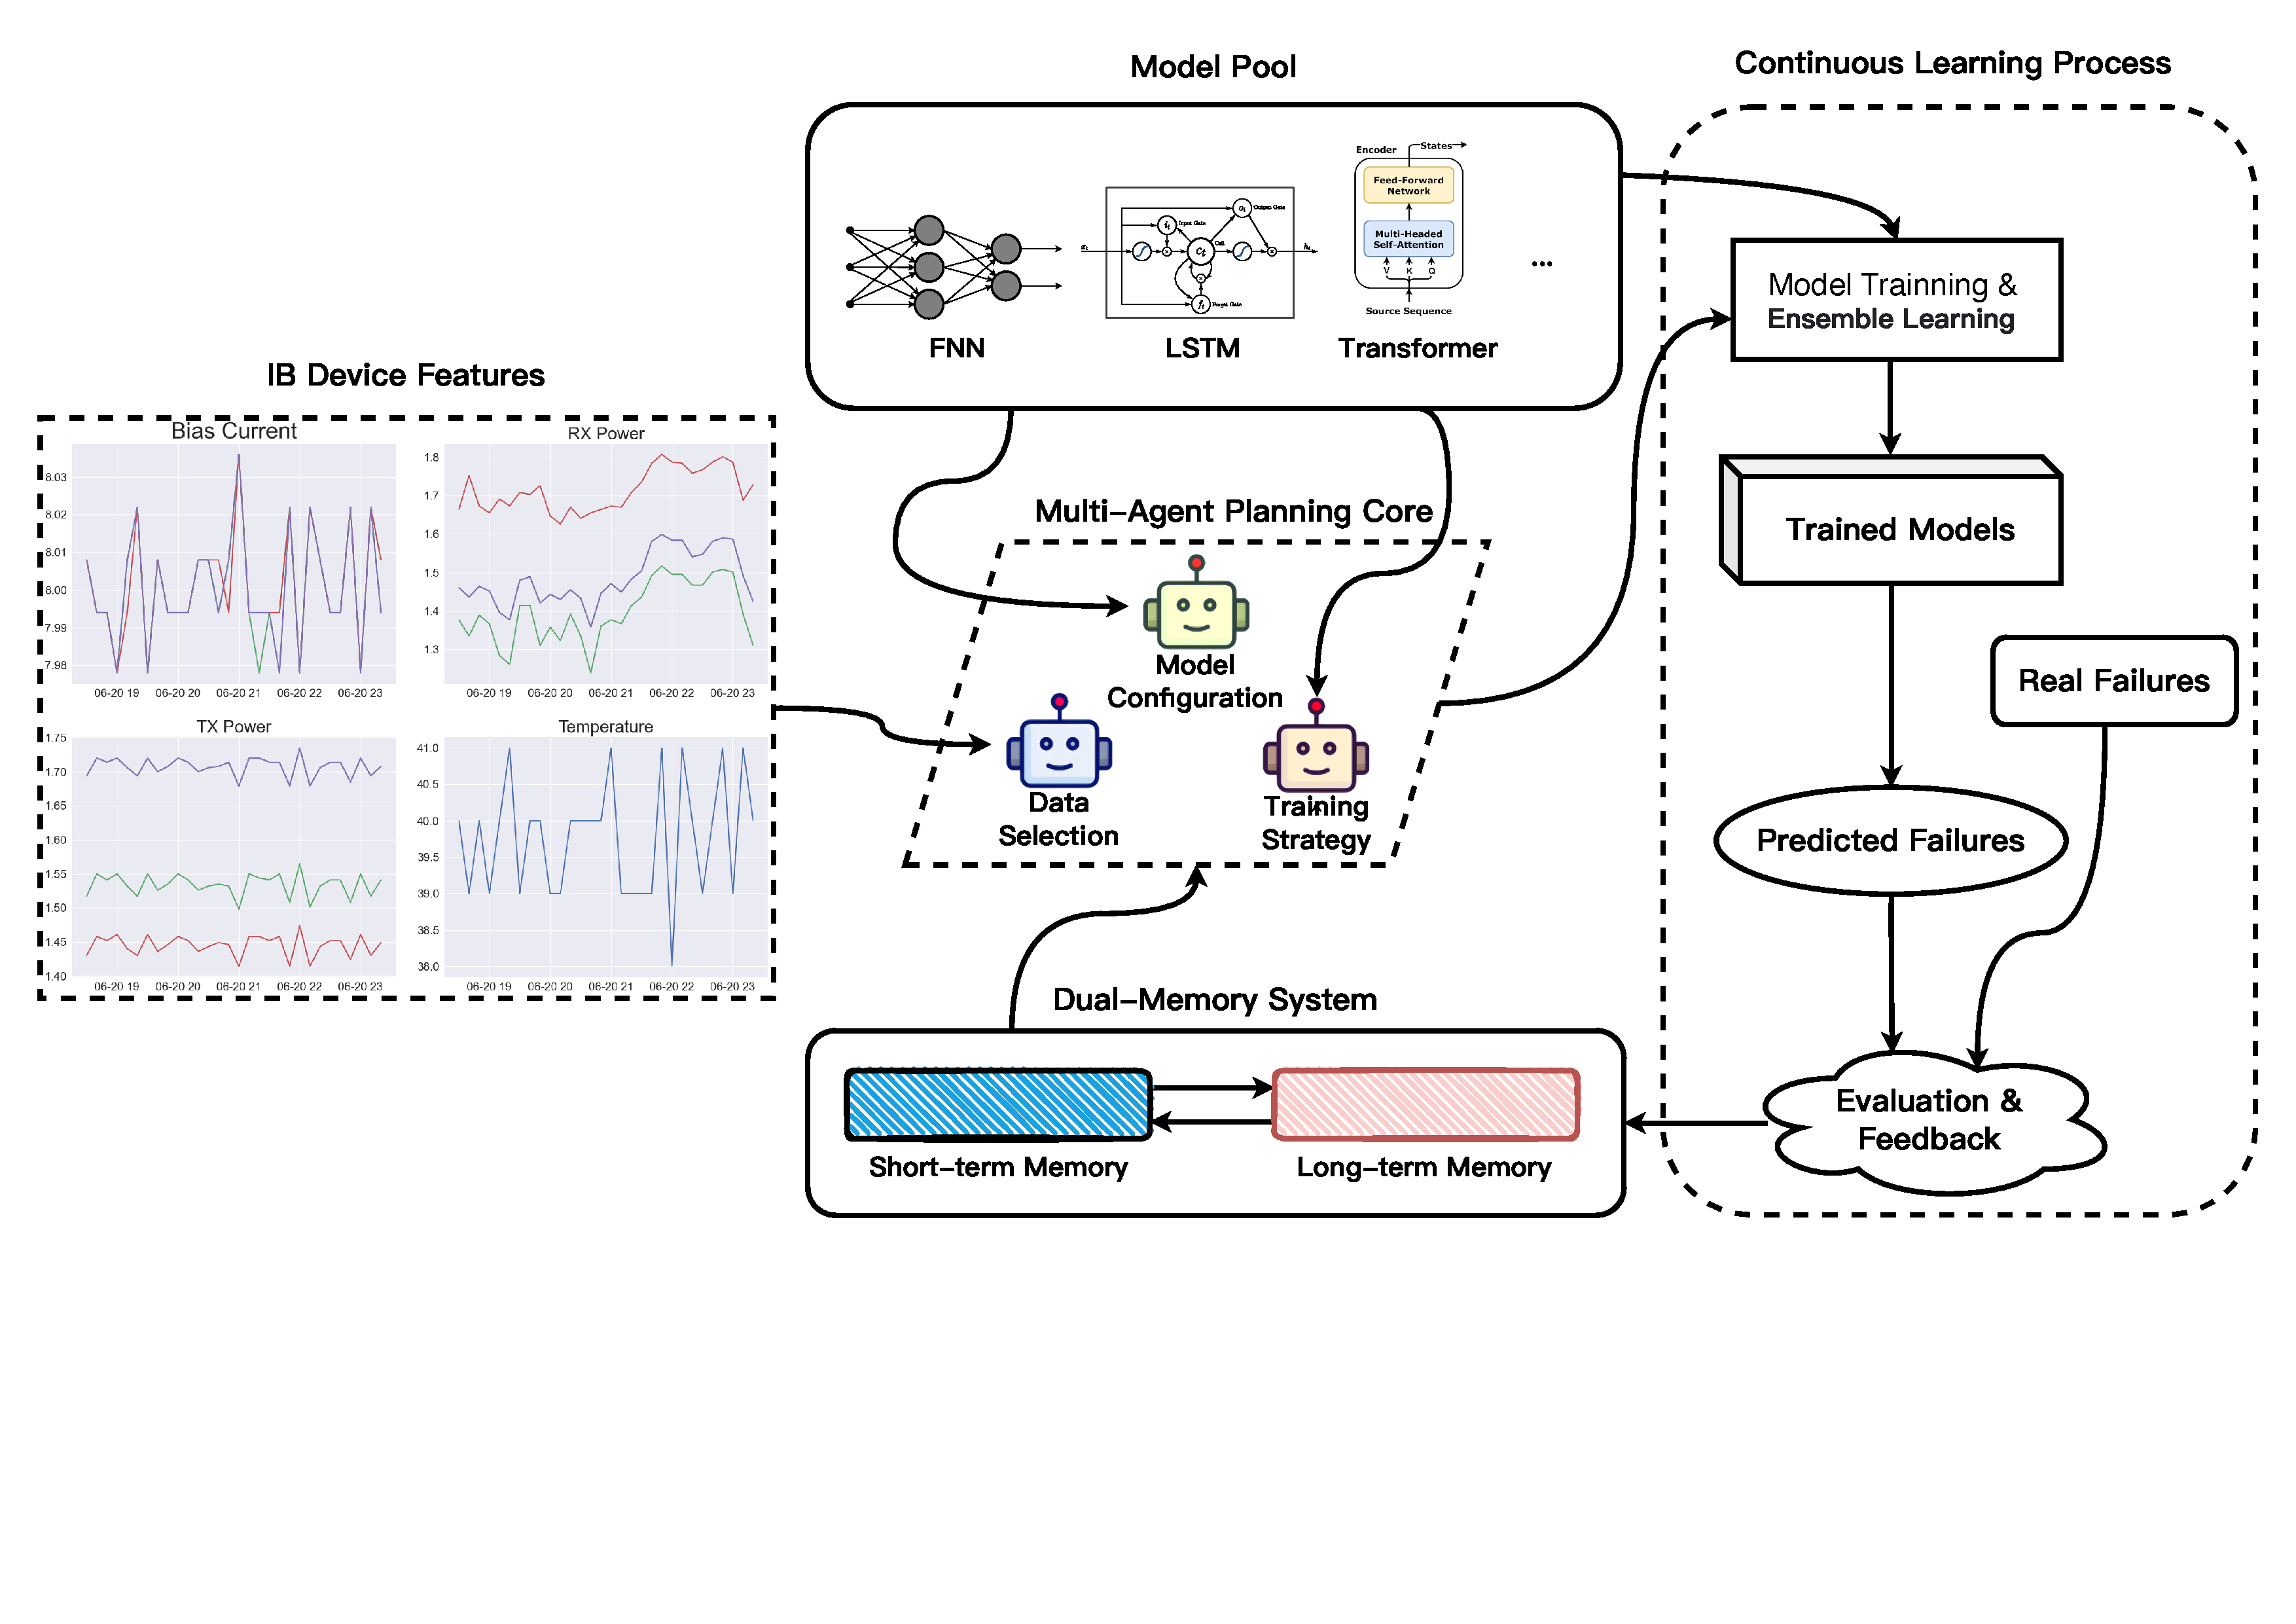
\includegraphics[width=0.95\textwidth]{fig/agent.pdf}
    \caption{Overview of SALCA-IB architecture. The system integrates (a) a model pool containing diverse deep learning models, (b) a multi-agent planning core for intelligent orchestration, (c) a dual-memory system for knowledge retention, and (d) a continuous learning process for adaptive optimization.}
    \label{fig:salca-ib}
\end{figure*}


\section{Related Work}

\subsection{HPC Clusters Failure Prediction}
Failure prediction in HPC clusters, particularly for large-scale GPU training workloads, has been extensively studied due to its critical importance in maintaining system reliability. Traditional approaches primarily rely on statistical methods and machine learning models. He et al. \cite{b6} analyzed hardware failures in deep learning training systems and found that GPU failures significantly impact training progress and model convergence. Similarly, Liu et al. \cite{b8} focused specifically on predicting GPU failures under intensive deep learning workloads, highlighting the unique challenges of monitoring and predicting failures in GPU-heavy computing environments.

More recent work has attempted to address these challenges through ensemble methods and deep learning approaches. Nie et al. \cite{b10} introduced GPU error prediction models using temporal and spatial dependencies to improve prediction robustness under limited data conditions, which shares similarities with our model pool concept but lacks intelligent orchestration. Das et al. \cite{b5} explored LSTM-based deep learning techniques to predict system health and lead times to failure, conceptually related to our long-term memory mechanism but without continuous adaptation capabilities. Liu et al. \cite{b8} further advanced GPU failure prediction using high-precision methods under deep learning workloads, demonstrating improved accuracy but still facing challenges in dynamic environments. Despite these advances, as highlighted by Alharthi et al. \cite{b2}, existing methods still face significant challenges in handling dynamic network environments and maintaining long-term prediction accuracy.

\subsection{LLM-based Reasoning, Memory and Self-Refinement}
Recent advances in LLM capabilities have opened new possibilities for complex reasoning and decision-making tasks. These developments can be examined across three key aspects:

\subsubsection{Reasoning and Verification}
LLMs have demonstrated remarkable capabilities in complex reasoning, though with certain limitations. Chen et al. \cite{chen2023} established the effectiveness of chain-of-thought prompting for enhancing reasoning abilities, while Wang et al. \cite{wang2023} advanced this further through a self-consistency framework that validates multiple reasoning paths. However, Tyen et al. \cite{tyen2023} revealed a critical limitation: while LLMs excel at correction with guidance, they struggle with autonomous error detection. Weng et al. \cite{weng2023} addressed this challenge by developing self-verification mechanisms that significantly improve reasoning reliability.

\subsubsection{Memory Integration}
The integration of external memory mechanisms has emerged as a crucial enhancement to LLM capabilities. Krishnamurthy et al. \cite{krishnamurthy2023} pioneered a hierarchical memory architecture that effectively manages both short-term and long-term knowledge retention. This approach was complemented by Li et al. \cite{li2023}, who developed an adaptive memory pruning mechanism that optimizes memory efficiency while preserving critical information. For domain-specific applications, Zhang et al. \cite{zhang2023} demonstrated successful integration of external knowledge bases with LLMs, while Shridhar et al. \cite{shridhar2023} proposed the ART framework for intelligent output refinement.

\subsubsection{Continuous Learning and Adaptation}
Recent research has focused on enhancing LLMs' ability to learn and adapt continuously. Kumar et al. \cite{kumar2023} developed a self-improving framework where LLMs generate and evaluate their own optimization strategies. This work was extended by Liu et al. \cite{liu2023}, who introduced an iterative refinement mechanism using structured feedback loops. Zhao et al. \cite{zhao2023} further advanced this field through a meta-learning approach that enables strategy adaptation based on task-specific feedback.

While these advances demonstrate significant progress in LLM capabilities, their application to network failure prediction remains largely unexplored, particularly in addressing the challenges of dynamic network environments and real-time adaptation requirements.

\section{Methodology}

SALCA-IB is designed as a self-adaptive intelligent system that leverages large language models (LLMs) to orchestrate network failure prediction in industrial blockchain environments. As illustrated in Fig. \ref{fig:salca-ib}, the system integrates four key components: an LLM-driven planning core, a dual-memory system, a deep learning model pool, and a continuous learning process.

As shown in Algorithm \ref{alg:salca-ib}, the LLM planning core serves as the system's central intelligence, orchestrating model selection, data processing, and strategy optimization. The dual-memory system combines short-term memory for rapid response and long-term memory for knowledge retention, enabling both immediate adaptation and sustained optimization. The model pool comprises diverse deep learning models (MLP, LSTM, and Transformer) that serve as the execution layer for failure prediction. Through continuous learning, the system evaluates prediction outcomes and adjusts strategies dynamically, ensuring robust performance in evolving network conditions. The detailed design of each component is elaborated in the following sections.

\subsection{LLM-Driven Planning Core}
Traditional failure prediction systems often rely on static model architectures and fixed training strategies, limiting their effectiveness in dynamic IB environments. Our LLM-driven planning core addresses this challenge by orchestrating three key components: data selection, model configuration, and training strategy optimization, as shown in Fig. \ref{fig:salca-ib}.

\subsubsection{Data Selection}
The data selection module processes IB network data streams $\mathcal{D} = \{(X_t, y_t)\}_{t=1}^T$, where $X_t \in \mathbb{R}^{w \times d}$ represents a sequence of network states within a sliding window. Specifically, $X_t = [x_{t-w+1}, ..., x_t]$ where $x_i \in \mathbb{R}^d$ contains $d$ network features at time step $i$, $w$ is the window size (e.g., 30 time steps), and $y_t \in \{0,1\}$ indicates whether a failure occurs following this sequence. Given historical knowledge $\mathcal{K} \subset Mem_{long}$, the LLM performs reasoning-based selection through:

\begin{equation}
    \mathcal{D}_{train} = f_{LLM}(\mathcal{D}, \mathcal{K}) = \{(X_i, y_i) | s_i > \tau, (X_i, y_i) \in \mathcal{D}\}
\end{equation}

where $s_i$ is the sequence importance score determined by LLM reasoning:
\begin{equation}
    s_i = LLM(X_i, \mathcal{K}, \text{prompt}_{select})
\end{equation}

The LLM generates importance scores through a structured reasoning process that evaluates both temporal evolution patterns and feature interactions within each sequence. This evaluation process is guided by carefully designed prompts that encode domain knowledge about network failure progression patterns and their manifestation across multiple features over time.

The data selection process consists of three sequential components:

\textit{a) Temporal Window Selection}: The LLM analyzes temporal context to determine optimal window configuration:
\begin{equation}
    W_t^* = LLM(\{X_{t-k}, ..., X_t\}, \mathcal{K}, \text{prompt}_{temporal})
\end{equation}
where $\text{prompt}_{temporal}$ guides the analysis of multi-scale temporal dependencies. The window selection considers both the granularity of individual time steps and the overall sequence length needed to capture failure progression patterns.

\textit{b) Distribution Assessment}: For selected windows, the LLM evaluates sequence representativeness:
\begin{equation}
    q_i = LLM(X_i, W_t^*, \mathcal{K}, \text{prompt}_{distribution})
\end{equation}
This assessment examines both the temporal evolution of individual features and their cross-feature correlations within each sequence. The evaluation particularly focuses on identifying characteristic patterns that historically preceded failure events.

\textit{c) Final Selection}: The LLM integrates previous analyses for final sequence selection:
\begin{equation}
    \mathcal{D}_{train} = \{(X_i, y_i) | LLM(q_i, \mathcal{K}, \text{prompt}_{final}) > \tau\}
\end{equation}
The final selection phase considers the completeness and quality of feature sequences, ensuring selected samples contain meaningful progression patterns for failure prediction.

The prompt design for each component incorporates specific aspects of temporal sequence analysis and feature interaction patterns. This enables the LLM to identify and select sequences that best capture the progression of network states leading to potential failures, while considering both historical patterns and current network conditions.

\subsubsection{Model Configuration}
The model configuration module dynamically selects and configures prediction models based on both current data characteristics and historical performance patterns. Given a model pool $\mathcal{M} = \{M_1, ..., M_m\}$ containing various neural architectures (e.g.,CNN, LSTM, Transformer), the LLM performs configuration through:

\begin{equation}
    (M_{selected}, \Theta, S) = f_{LLM}^{config}(\mathcal{M}, \mathcal{K}, X_t)
\end{equation}

where $M_{selected} \subset \mathcal{M}$ is the selected model subset, $\Theta$ represents their corresponding parameter configurations, and $S$ defines the ensemble strategy. The configuration process consists of three key components:

\textit{a) Architecture Selection}: The LLM evaluates and selects appropriate model architectures based on current sequence characteristics:
\begin{equation}
    M_{selected} = LLM(\mathcal{M}, X_t, \mathcal{K}, \text{prompt}_{arch})
\end{equation}
This selection considers the temporal dependency patterns in $X_t$, such as choosing LSTM for strong short-term dependencies or Transformer for capturing long-range correlations. The historical performance records in $\mathcal{K}$ guide this selection by providing evidence of each architecture's effectiveness under similar conditions.

\textit{b) Parameter Configuration}: For each selected model $M_i \in M_{selected}$, the LLM determines its optimal configuration:
\begin{equation}
    \theta_i = LLM(M_i, X_t, \mathcal{K}, \text{prompt}_{param})
\end{equation}
where $\theta_i \in \Theta$ includes both architectural parameters (e.g., number of layers, hidden dimensions) and training parameters (e.g., learning rate, batch size). The configuration is based on both the current data characteristics and historical configuration effectiveness stored in $\mathcal{K}$.

\textit{c) Ensemble Strategy Design}: The LLM designs an ensemble strategy $S$ that optimally combines the selected models:
\begin{equation}
    S = LLM(M_{selected}, \Theta, \mathcal{K}, \text{prompt}_{ensemble})
\end{equation}
The ensemble strategy includes both the voting mechanism and individual model weights, determined by analyzing each model's historical reliability and current data fitness. The final ensemble model is constructed as:
\begin{equation}
    M_{ensemble}(X_t) = \sum_{i=1}^{|M_{selected}|} w_i M_i(X_t; \theta_i)
\end{equation}
where $w_i$ represents the dynamic weight assigned to each model's prediction.

This knowledge-driven configuration process enables the system to adapt its prediction models dynamically based on evolving network conditions while leveraging accumulated experience from historical operations.

\subsubsection{Training Strategy}
The training strategy module optimizes the learning process of the ensemble model through LLM-driven adaptation. Given the selected training data $\mathcal{D}_{train}$ and configured ensemble model $M_{ensemble}$, the training process is formulated as:

\begin{equation}
    M_{ensemble}^* = f_{LLM}^{train}(M_{ensemble}, \mathcal{D}_{train}, \mathcal{K})
\end{equation}

The training optimization process consists of three key components:

\textit{a) Initial Parameter Configuration}: For each model $M_i$ in the ensemble, the LLM determines optimal training parameters based on historical experience:
\begin{equation}
    \{\eta_i, B_i\} = LLM(M_i, \mathcal{D}_{train}, \mathcal{K}, \text{prompt}_{init})
\end{equation}
where $\eta_i$ is the fixed learning rate and $B_i$ is the batch size for model $M_i$. These parameters remain constant throughout the training process, with their values determined by analyzing historical training patterns stored in $\mathcal{K}$.

\textit{b) Loss Function Design}: The LLM constructs a composite loss function based on prediction requirements and historical error patterns:
\begin{equation}
    \begin{aligned} 
    \mathcal{L}(X_t, y_t) = \alpha\mathcal{L}_{ce}(X_t, y_t) &+ \beta\mathcal{L}_{temporal}(X_t) \\
    &+ \gamma\mathcal{L}_{reg}(M_{ensemble})
    \end{aligned}
\end{equation}
where $\mathcal{L}_{ce}$ is the cross-entropy loss for failure prediction, $\mathcal{L}_{temporal}$ penalizes temporal inconsistency in predictions, and $\mathcal{L}_{reg}$ provides regularization based on historical failure patterns. The weights $\alpha, \beta, \gamma$ are determined before training:
\begin{equation}
    [\alpha, \beta, \gamma] = LLM(\mathcal{D}_{train}, \mathcal{K}, \text{prompt}_{loss})
\end{equation}

\textit{c) Performance Monitoring}: The LLM continuously evaluates prediction performance and triggers model updates when necessary:
\begin{equation}
    \delta_t = LLM(M_{ensemble}, X_t, \mathcal{K}, \text{prompt}_{monitor})
\end{equation}
where $\delta_t$ is the update decision signal. When significant performance degradation is detected, the system initiates retraining with newly configured parameters:
\begin{equation}
    M_{ensemble}^{t+1} = \begin{cases}
        \text{Retrain}(M_{ensemble}, \mathcal{D}_{new}, \{\eta_i^{new}\}) & \text{if } \delta_t > \tau \\
        M_{ensemble}^t & \text{otherwise}
    \end{cases}
\end{equation}

This framework ensures stable training processes while maintaining the flexibility to adapt to significant changes in network conditions through model retraining with newly optimized parameters.

\subsection{Dual-Memory System}
The dual-memory system implements a JSON-based knowledge repository that facilitates efficient experience accumulation and retrieval for LLM-driven decision making. This system addresses the context length limitations of LLMs while enabling continuous learning through structured knowledge preservation.

\subsubsection{Memory Architecture}
The short-term memory maintains a dynamic operational context for immediate decision support:
\begin{equation}
    Mem_{short} = \{F_{current}, T_{range}, P_{model}, M_{config}, F_{recent}\}
\end{equation}
where $F_{current}$ represents the active feature set with selection rationale, $T_{range}$ captures temporal context with start and end timestamps, $P_{model}$ stores recent model performance metrics, and $M_{config}$ maintains current model configurations and ensemble strategies.

The long-term memory implements a persistent knowledge base with activation tracking:
\begin{equation}
    Mem_{long} = \{F_{stats}, M_{history}, E_{record}, A_{track}, F_{history}\}
\end{equation}
where $F_{stats}$ maintains feature statistics and selection history, $M_{history}$ records successful model configurations, $E_{record}$ stores historical experience entries, $A_{track}$ tracks memory activation patterns, and $F_{history}$ maintains valuable historical feedback:
\begin{equation}
    F_{history} = \{(f_i, t_i, e_i) | Q(f_i) > \tau_{feedback}\}
\end{equation}

Each feedback entry contains:
\begin{equation}
    f_i = \{P_i, R_i, A_i\}
\end{equation}
where $P_i$ represents performance metrics, $R_i$ captures LLM reasoning, and $A_i$ records adaptation decisions.

\subsubsection{Memory Operations}
The system implements three basic memory operations:

\textit{a) Experience Recording}: The system records new operational experiences in short-term memory:
\begin{equation}
    Mem_{short}^{t+1} = Record(X_t, y_t, P_t, C_t)
\end{equation}
where $X_t$ represents current feature data, $y_t$ is the prediction outcome, $P_t$ contains performance metrics, and $C_t$ includes current configurations.

\textit{b) Memory Transfer}: The system periodically transfers valuable experiences from short-term to long-term memory:
\begin{equation}
    Mem_{long}^{t+1} = Transfer(Mem_{short}, Mem_{long})
\end{equation}
This operation includes recording successful feature selections, model configurations, and performance patterns.

\textit{c) Activation-based Cleanup}: The system implements an activation-aware cleanup mechanism:
\begin{equation}
    A_{score}(e_i) = \lambda\frac{t_{current} - t_{last}(e_i)}{T_{max}} + (1-\lambda)\frac{n_{access}(e_i)}{N_{max}}
\end{equation}
where $\lambda$ balances recency and frequency of access. The cleanup operation removes entries based on their activation scores:
\begin{equation}
    Mem_{clean} = \{e_i | A_{score}(e_i) > \tau_{active}\}
\end{equation}
where $\tau_{active}$ is the retention threshold.

The system maintains its effectiveness through activation-aware memory management, ensuring both efficiency and relevance in supporting LLM-driven decisions.
    
\subsection{Continuous Learning Process}
The continuous learning process implements a self-evolving mechanism through LLM-driven optimization and structured feedback analysis. This process establishes a closed-loop learning cycle that continuously refines prediction capabilities based on operational experiences.

\subsubsection{Performance-Driven Feedback Generation}
The system generates structured feedback based on actual prediction results:
\begin{equation}
    P_t = \{accuracy_t, precision_t, recall_t, stability_t\}
\end{equation}
where performance metrics are analyzed through LLM reasoning to generate comprehensive feedback:
\begin{equation}
    f_t = LLM(P_t, E_{record}, \text{prompt}_{analyze})
\end{equation}
The feedback contains component-wise assessments:
\begin{equation}
    f_t = \{(c_i, s_i, r_i) | c_i \in \{feature, model, training\}\}
\end{equation}
where $s_i$ indicates performance status and $r_i$ provides specific improvement recommendations.

\subsubsection{Actionable Improvement Strategy}
Based on the feedback analysis, the system generates concrete improvement strategies:
\begin{equation}
    I_t = LLM(f_t, F_{history}, \text{prompt}_{improve})
\end{equation}
where $I_t$ specifies actionable adjustments:
\begin{equation}
    I_t = \{(a_i, p_i, \Delta_i) | a_i \in Actions\}
\end{equation}
Here, $a_i$ represents specific actions, $p_i$ indicates their priority, and $\Delta_i$ defines the adjustment magnitude.

\subsubsection{Self-Refinement Process}
The system implements a three-stage refinement process:

\textit{a) Strategy Validation}: Proposed improvements are validated against historical experiences:
\begin{equation}
    V_t = LLM(I_t, F_{history}, \text{prompt}_{validate})
\end{equation}

\textit{b) Component Optimization}: Validated strategies are applied to system components:
\begin{equation}
    C_{t+1} = Optimize(C_t, V_t, \text{prompt}_{refine})
\end{equation}
where $C_t$ represents the current configuration of features, models, or training parameters.

\textit{c) Effectiveness Assessment}: The system evaluates optimization outcomes:
\begin{equation}
    E_t = Assess(C_{t+1}, P_{t+1}, \text{prompt}_{assess})
\end{equation}

The assessment results are integrated into the feedback history to guide future improvements:
\begin{equation}
    F_{history}^{t+1} = Update(F_{history}, E_t, \text{prompt}_{update})
\end{equation}

This closed-loop self-refining process and its integration with the dual-memory system ensures continuous improvement while maintaining operational efficiency through experience-based optimization.

The overall framework is summarized in Algorithm \ref{alg:salca-ib}.



\section{Experimental Evaluation}

\subsection{Dataset Construction and Collection}

\subsubsection{Infrastructure Overview}
Our experimental environment consists of a large-scale InfiniBand cluster designed for high-performance computing workloads, particularly focused on training large language models exceeding 200 billion parameters. Such training tasks demand exceptional network performance and reliability, as network failures can significantly impact model convergence and training efficiency. The cluster implements a two-layer Leaf-Spine topology with full-mesh connectivity, comprising 2048 computing cards distributed across 8 pods. Each pod contains 256 cards connected through 8 LEAF switches, with the overall network infrastructure including 64 Leaf switches and 32 Spine switches. This architecture, compliant with NVIDIA's rail-optimized specifications, ensures optimal bandwidth utilization and minimal communication latency while maintaining network redundancy, which is crucial for sustaining the massive data transfers required in distributed LLM training.

Through our analysis, we identified two primary categories of network failures in this infrastructure: link flapping and complete link down events. These failures are particularly critical in LLM training scenarios, where even brief network interruptions can lead to significant training delays or potential loss of computation resources. The failures typically originate from optical module degradation under sustained exposure to adverse environmental conditions, particularly in scenarios involving high-temperature operation and sustained high workloads characteristic of intensive LLM training operations. 

\subsubsection{Data Collection}
We developed a comprehensive data collection framework that integrates four complementary monitoring approaches. System performance counters provide detailed insights into network interface card (NIC) performance and local link status. The OpenSM subnet manager logs capture network-wide connectivity status and state transitions across all devices. Hardware diagnostics data collected through management interfaces provides information about physical components including NICs, optical modules, and cables. Additionally, network topology information is gathered to maintain a complete map of physical connections between devices. 

The final processed dataset demonstrates significant scale and comprehensiveness. The performance metrics data includes approximately 77.8 billion data points collected over eight months, comprising 55 metrics per InfiniBand card (36 performance and error diagnostic metrics, 2 temperature indicators, and 17 physical parameters) collected from 256 nodes, each equipped with 8 IB cards, sampled twice per minute. Real-time state snapshots contribute an additional 40 million records, capturing every network state change. The OpenSM subnet manager logs contain 20.18 million entries documenting network events and state transitions. 

For the failure prediction task, we employ a similar sampling strategy with Liu et al. \cite{b8} for training and evaluation phases. During training, we maintain a balanced 1:1 ratio between failure and normal samples to ensure the model learns effectively from both classes. For evaluation and real-world prediction scenarios, we use a more realistic 1:8 ratio that better reflects the natural distribution of failure events in production environments. 

\subsection{Experimental Setup}

\subsubsection{Implementation Details}
To investigate how LLM reasoning capabilities affect the performance of our SALCA-IB framework, we conducted experiments with four different large language models: GPT-4o (accessed via OpenAI's API), Llama-3-70B-Instruct, Yi-1.5-34B-Chat, and Qwen2.5-14B-Instruct. Each experiment uses a single LLM as the reasoning engine throughout the entire process, allowing us to evaluate how models of different sizes and reasoning capabilities impact the framework's effectiveness. The locally deployed models (Llama-3, Yi-1.5, and Qwen2.5) run on Nvidia H100 GPUs using vLLM for optimized inference.

The prediction model pool consists of lightweight neural networks optimized for CPU inference. These models were trained on our IB network dataset using CPU resources to ensure efficient deployment in production environments. Table \ref{tab:model_config} shows the configuration search space and LLM selection examples.

\begin{table}[!t]
\caption{Model Pool Configuration Options with LLM Selection Examples}
\label{tab:model_config}
\begin{center}
\begin{tabular}{|p{2.5cm}|p{5cm}|}
\hline
\multicolumn{2}{|c|}{\textbf{Model Architecture Parameters}} \\
\hline
\textbf{Model Type} & \textbf{Parameter Range (Example Choice)} \\
\hline
\multirow{4}{*}{MLP} & Layers: [3-6] (4) \\
& Units: [64,128,256,512] (128) \\
& Dropout: [0.1-0.5] (0.3) \\
& Width decay ratio: [1.5-3.0] (2.0) \\
\hline
\multirow{4}{*}{CNN} & Conv layers: [1-5] (3) \\
& Filters: [32,64,128] (64) \\
& Kernel size: [3,5,7] (3) \\
& Pooling: [Max, Average] (Max) \\
\hline
\multirow{4}{*}{LSTM} & Layers: [1-8] (4) \\
& Hidden units: [64,128,256,512] (128) \\
& Dropout: [0.1-0.5] (0.4) \\
& Sequence length: [10-50] (30) \\
\hline
\multirow{4}{*}{GRU} & Layers: [1-4] (3) \\
& Hidden units: [64,128,256,512] (256) \\
& Dropout: [0.1-0.5] (0.3) \\
& Update gate bias: [-2.0,2.0] (1.0) \\
\hline
\multirow{4}{*}{Transformer} & Layers: [2-8] (6) \\
& Embedding dim: [128,256,512] (256) \\
& Dropout: [0.1-0.5] (0.5) \\
& Attention heads: [4,8,16] (8) \\
\hline
\multicolumn{2}{|c|}{\textbf{Training Parameters}} \\
\hline
\multicolumn{2}{|l|}{Batch size: [32-512] (64)} \\
\multicolumn{2}{|l|}{Learning rate: [1e-5, 1e-4, 1e-3] (5e-4)} \\
\multicolumn{2}{|l|}{Optimizer: AdamW with weight decay [1e-5, 1e-3] (1e-4)} \\
\multicolumn{2}{|l|}{Early stopping patience: [5-20 epochs] (10)} \\
\hline
\end{tabular}
\end{center}
\end{table}

\subsubsection{Baseline Methods}
We designed three categories of baseline methods to evaluate the effectiveness of our SALCA-IB framework:

\textbf{Individual Deep Learning Models:} We first evaluated each model from our model pool independently. The MLP model serves as a basic deep learning baseline with its hierarchical feature extraction capability. The LSTM and GRU models represent sequence modeling approaches that capture temporal dependencies in network states. The Transformer model provides a self-attention based baseline that can model long-range dependencies. The CNN model is included to capture spatial hierarchies and local patterns in the data, which can be particularly useful for identifying localized anomalies. Each model was trained with its optimal configuration as determined by grid search.

\textbf{Traditional Ensemble Methods:} We then combined these deep learning models using conventional ensemble strategies:
(1) Majority Voting, where each model contributes equally to the final prediction;
(2) Weighted Voting, where weights are assigned based on each model's validation performance;
These ensemble methods represent traditional approaches to model combination without dynamic adaptation.

\textbf{LLM-based Methods:} To isolate the contribution of LLM orchestration, we implemented several LLM-based approaches using the same set of base models. These include End-to-End prompting, Chain-of-Thought prompting \cite{chen2023}, and Self-Refine \cite{madaan2023}. For consistency and fair comparison, each method was tested using the GPT-4o API, aligning with SALCA-IB's LLM-driven orchestration mechanism.

\subsection{Evaluation Methodology}

\subsubsection{Evaluation Objectives}
The primary objective of our evaluation is to demonstrate the superiority of SALCA-IB over traditional methods in both static and dynamic network environments. We focus on two key scenarios: the static scenario, which evaluates performance within a fixed time period to assess immediate prediction accuracy, and the dynamic scenario, which evaluates performance across extended time periods to assess adaptability to network feature distribution changes.

\subsubsection{Experimental Protocol}
Experiments were conducted using an 8-month dataset from our production IB network. In the static scenario, models are trained and evaluated within a single, fixed time window, with performance metrics including Precision@K, Recall@K, and F1@K. In contrast, the dynamic scenario involves training models on initial data and evaluating them over subsequent time windows to simulate real-world conditions. Controlled perturbations are introduced to network features to mimic distribution shifts, with performance metrics focusing on adaptability, including changes in F1@K over time.

\subsubsection{Evaluation Metrics}
We employ ranking-based metrics with K set to 2\% of total instances. Precision@K, Recall@K, and F1@K are used to evaluate prediction performance, particularly under resource constraints and class imbalance. These metrics are defined as follows: Precision@K is the ratio of true positives to the sum of true positives and false positives within the top K predictions. Recall@K is the ratio of true positives to the sum of true positives and false negatives within the top K predictions. F1@K is the harmonic mean of Precision@K and Recall@K.

All experiments are repeated 5 times with different random seeds to ensure statistical significance, and the mean values and standard deviations are reported.

\begin{table*}[!t]
\caption{Performance Comparison of Different Methods on IB Network Failure Prediction}
\label{tab:main_results}
\renewcommand{\arraystretch}{1.2}
\centering
\begin{tabular}{l|ccc|ccc}
\hline
\multirow{2}{*}{\textbf{Method}} & \multicolumn{3}{c|}{\textbf{Static Scenario}} & \multicolumn{3}{c}{\textbf{Dynamic Scenario}} \\
\cline{2-7}
& P@K (\%) & R@K (\%) & F1@K (\%) & P@K (\%) & R@K (\%) & F1@K (\%) \\
\hline
\multicolumn{7}{l}{\textit{Individual Models}} \\
\hline
FNN & 72.3±1.2 & 68.5±1.4 & 70.3±1.3 & 65.2±2.1 & 61.8±2.3 & 63.4±2.2 \\
LSTM & 75.6±1.1 & 71.2±1.3 & 73.3±1.2 & 68.4±1.9 & 64.5±2.1 & 66.4±2.0 \\
GRU & 76.1±1.0 & 72.4±1.2 & 74.2±1.1 & 69.2±1.8 & 65.7±2.0 & 67.4±1.9 \\
Transformer & 77.3±0.9 & 73.8±1.1 & 75.5±1.0 & 70.5±1.7 & 66.9±1.9 & 68.6±1.8 \\
CNN & 74.8±1.3 & 70.6±1.5 & 72.6±1.4 & 67.3±2.2 & 63.5±2.4 & 65.3±2.3 \\
\hline
\multicolumn{7}{l}{\textit{Traditional Ensemble Methods}} \\
\hline
Majority Voting & 78.5±0.8 & 74.9±1.0 & 76.6±0.9 & 71.8±1.6 & 68.2±1.8 & 69.9±1.7 \\
Weighted Voting & 79.2±0.7 & 75.6±0.9 & 77.3±0.8 & 72.6±1.5 & 69.0±1.7 & 70.7±1.6 \\
\hline
\multicolumn{7}{l}{\textit{LLM-based Methods (with GPT-4o)}} \\
\hline
End-to-End Prompting & 80.1±0.6 & 76.4±0.8 & 78.2±0.7 & 74.3±1.4 & 70.8±1.6 & 72.5±1.5 \\
Chain-of-Thought & 80.8±0.5 & 77.1±0.7 & 78.9±0.6 & 75.0±1.3 & 71.5±1.5 & 73.2±1.4 \\
Self-Refine & 81.3±0.5 & 77.6±0.7 & 79.4±0.6 & 75.7±1.2 & 72.2±1.4 & 73.9±1.3 \\
\hline
\multicolumn{7}{l}{\textit{SALCA-IB with Different LLM Cores}} \\
\hline
SALCA-IB (Qwen2.5-14B) & 82.1±0.5 & 78.4±0.7 & 80.2±0.6 & 77.3±1.2 & 73.8±1.4 & 75.5±1.3 \\
SALCA-IB (Yi-1.5-34B) & 82.8±0.5 & 79.1±0.6 & 80.9±0.5 & 78.5±1.1 & 75.0±1.3 & 76.71.2 \\
SALCA-IB (Llama-3-70B) & 83.6±0.4 & 79.9±0.6 & 81.7±0.5 & 79.8±1.0 & 76.4±1.2 & 78.1±1.1 \\
\textbf{SALCA-IB (GPT-4o)} & \textbf{84.5±0.4} & \textbf{80.8±0.6} & \textbf{82.6±0.5} & \textbf{81.2±1.0} & \textbf{77.9±1.2} & \textbf{79.5±1.1} \\
\hline
\end{tabular}
\end{table*}

\subsubsection{Main Results}
The results demonstrate that SALCA-IB significantly outperforms traditional methods, with a 6.8\% improvement in F1@K-score in static scenarios and a 15.9\% increase in dynamic scenarios. This highlights the framework's superior adaptability to changes in network feature distributions, validating its effectiveness in real-world applications.

\section{Ease of Use}

\subsection{Maintaining the Integrity of the Specifications}

The IEEEtran class file is used to format your paper and style the text. All margins, 
column widths, line spaces, and text fonts are prescribed; please do not 
alter them. You may note peculiarities. For example, the head margin
measures proportionately more than is customary. This measurement 
and others are deliberate, using specifications that anticipate your paper 
as one part of the entire proceedings, and not as an independent document. 
Please do not revise any of the current designations.

\section{Prepare Your Paper Before Styling}
Before you begin to format your paper, first write and save the content as a 
separate text file. Complete all content and organizational editing before 
formatting. Please note sections \ref{AA}--\ref{SCM} below for more information on 
proofreading, spelling and grammar.

Keep your text and graphic files separate until after the text has been 
formatted and styled. Do not number text heads---{\LaTeX} will do that 
for you.

\subsection{Abbreviations and Acronyms}\label{AA}
Define abbreviations and acronyms the first time they are used in the text, 
even after they have been defined in the abstract. Abbreviations such as 
IEEE, SI, MKS, CGS, ac, dc, and rms do not have to be defined. Do not use 
abbreviations in the title or heads unless they are unavoidable.

\subsection{Units}
\begin{itemize}
\item Use either SI (MKS) or CGS as primary units. (SI units are encouraged.) English units may be used as secondary units (in parentheses). An exception would be the use of English units as identifiers in trade, such as ``3.5-inch disk drive''.
\item Avoid combining SI and CGS units, such as current in amperes and magnetic field in oersteds. This often leads to confusion because equations do not balance dimensionally. If you must use mixed units, clearly state the units for each quantity that you use in an equation.
\item Do not mix complete spellings and abbreviations of units: ``Wb/m\textsuperscript{2}'' or ``webers per square meter'', not ``webers/m\textsuperscript{2}''. Spell out units when they appear in text: ``. . . a few henries'', not ``. . . a few H''.
\item Use a zero before decimal points: ``0.25'', not ``.25''. Use ``cm\textsuperscript{3}'', not ``cc''.)
\end{itemize}

\subsection{Equations}
Number equations consecutively. To make your 
equations more compact, you may use the solidus (~/~), the exp function, or 
appropriate exponents. Italicize Roman symbols for quantities and variables, 
but not Greek symbols. Use a long dash rather than a hyphen for a minus 
sign. Punctuate equations with commas or periods when they are part of a 
sentence, as in:
\begin{equation}
a+b=\gamma\label{eq}
\end{equation}

Be sure that the 
symbols in your equation have been defined before or immediately following 
the equation. Use ``\eqref{eq}'', not ``Eq.~\eqref{eq}'' or ``equation \eqref{eq}'', except at 
the beginning of a sentence: ``Equation \eqref{eq} is . . .''

\subsection{\LaTeX-Specific Advice}

Please use ``soft'' (e.g., \verb|\eqref{Eq}|) cross references instead
of ``hard'' references (e.g., \verb|(1)|). That will make it possible
to combine sections, add equations, or change the order of figures or
citations without having to go through the file line by line.

Please don't use the \verb|{eqnarray}| equation environment. Use
\verb|{align}| or \verb|{IEEEeqnarray}| instead. The \verb|{eqnarray}|
environment leaves unsightly spaces around relation symbols.

Please note that the \verb|{subequations}| environment in {\LaTeX}
will increment the main equation counter even when there are no
equation numbers displayed. If you forget that, you might write an
article in which the equation numbers skip from (17) to (20), causing
the copy editors to wonder if you've discovered a new method of
counting.

{\BibTeX} does not work by magic. It doesn't get the bibliographic
data from thin air but from .bib files. If you use {\BibTeX} to produce a
bibliography you must send the .bib files. 

{\LaTeX} can't read your mind. If you assign the same label to a
subsubsection and a table, you might find that Table I has been cross
referenced as Table IV-B3. 

{\LaTeX} does not have precognitive abilities. If you put a
\verb|\label| command before the command that updates the counter it's
supposed to be using, the label will pick up the last counter to be
cross referenced instead. In particular, a \verb|\label| command
should not go before the caption of a figure or a table.

Do not use \verb|\nonumber| inside the \verb|{array}| environment. It
will not stop equation numbers inside \verb|{array}| (there won't be
any anyway) and it might stop a wanted equation number in the
surrounding equation.

\subsection{Some Common Mistakes}\label{SCM}
\begin{itemize}
\item The word ``data'' is plural, not singular.
\item The subscript for the permeability of vacuum $\mu_{0}$, and other common scientific constants, is zero with subscript formatting, not a lowercase letter ``o''.
\item In American English, commas, semicolons, periods, question and exclamation marks are located within quotation marks only when a complete thought or name is cited, such as a title or full quotation. When quotation marks are used, instead of a bold or italic typeface, to highlight a word or phrase, punctuation should appear outside of the quotation marks. A parenthetical phrase or statement at the end of a sentence is punctuated outside of the closing parenthesis (like this). (A parenthetical sentence is punctuated within the parentheses.)
\item A graph within a graph is an ``inset'', not an ``insert''. The word alternatively is preferred to the word ``alternately'' (unless you really mean something that alternates).
\item Do not use the word ``essentially'' to mean ``approximately'' or ``effectively''.
\item In your paper title, if the words ``that uses'' can accurately replace the word ``using'', capitalize the ``u''; if not, keep using lower-cased.
\item Be aware of the different meanings of the homophones ``affect'' and ``effect'', ``complement'' and ``compliment'', ``discreet'' and ``discrete'', ``principal'' and ``principle''.
\item Do not confuse ``imply'' and ``infer''.
\item The prefix ``non'' is not a word; it should be joined to the word it modifies, usually without a hyphen.
\item There is no period after the ``et'' in the Latin abbreviation ``et al.''.
\item The abbreviation ``i.e.'' means ``that is'', and the abbreviation ``e.g.'' means ``for example''.
\end{itemize}
An excellent style manual for science writers is \cite{b7}.

\subsection{Authors and Affiliations}
\textbf{The class file is designed for, but not limited to, six authors.} A 
minimum of one author is required for all conference articles. Author names 
should be listed starting from left to right and then moving down to the 
next line. This is the author sequence that will be used in future citations 
and by indexing services. Names should not be listed in columns nor group by 
affiliation. Please keep your affiliations as succinct as possible (for 
example, do not differentiate among departments of the same organization).

\subsection{Identify the Headings}
Headings, or heads, are organizational devices that guide the reader through 
your paper. There are two types: component heads and text heads.

Component heads identify the different components of your paper and are not 
topically subordinate to each other. Examples include Acknowledgments and 
References and, for these, the correct style to use is ``Heading 5''. Use 
``figure caption'' for your Figure captions, and ``table head'' for your 
table title. Run-in heads, such as ``Abstract'', will require you to apply a 
style (in this case, italic) in addition to the style provided by the drop 
down menu to differentiate the head from the text.

Text heads organize the topics on a relational, hierarchical basis. For 
example, the paper title is the primary text head because all subsequent 
material relates and elaborates on this one topic. If there are two or more 
sub-topics, the next level head (uppercase Roman numerals) should be used 
and, conversely, if there are not at least two sub-topics, then no subheads 
should be introduced.

\subsection{Figures and Tables}
\paragraph{Positioning Figures and Tables} Place figures and tables at the top and 
bottom of columns. Avoid placing them in the middle of columns. Large 
figures and tables may span across both columns. Figure captions should be 
below the figures; table heads should appear above the tables. Insert 
figures and tables after they are cited in the text. Use the abbreviation 
``Fig.~\ref{fig}'', even at the beginning of a sentence.

\begin{table}[htbp]
\caption{Table Type Styles}
\begin{center}
\begin{tabular}{|c|c|c|c|}
\hline
\textbf{Table}&\multicolumn{3}{|c|}{\textbf{Table Column Head}} \\
\cline{2-4} 
\textbf{Head} & \textbf{\textit{Table column subhead}}& \textbf{\textit{Subhead}}& \textbf{\textit{Subhead}} \\
\hline
copy& More table copy$^{\mathrm{a}}$& &  \\
\hline
\multicolumn{4}{l}{$^{\mathrm{a}}$Sample of a Table footnote.}
\end{tabular}
\label{tab1}
\end{center}
\end{table}


Figure Labels: Use 8 point Times New Roman for Figure labels. Use words 
rather than symbols or abbreviations when writing Figure axis labels to 
avoid confusing the reader. As an example, write the quantity 
``Magnetization'', or ``Magnetization, M'', not just ``M''. If including 
units in the label, present them within parentheses. Do not label axes only 
with units. In the example, write ``Magnetization (A/m)'' or ``Magnetization 
\{A[m(1)]\}'', not just ``A/m''. Do not label axes with a ratio of 
quantities and units. For example, write ``Temperature (K)'', not 
``Temperature/K''.

\section*{Acknowledgment}

The preferred spelling of the word ``acknowledgment'' in America is without 
an ``e'' after the ``g''. Avoid the stilted expression ``one of us (R. B. 
G.) thanks $\ldots$''. Instead, try ``R. B. G. thanks$\ldots$''. Put sponsor 
acknowledgments in the unnumbered footnote on the first page.

\section*{References}

Please number citations consecutively within brackets \cite{b1}. The 
sentence punctuation follows the bracket \cite{b2}. Refer simply to the reference 
number, as in \cite{b3}---do not use ``Ref. \cite{b3}'' or ``reference \cite{b3}'' except at 
the beginning of a sentence: ``Reference \cite{b3} was the first $\ldots$''

Number footnotes separately in superscripts. Place the actual footnote at 
the bottom of the column in which it was cited. Do not put footnotes in the 
abstract or reference list. Use letters for table footnotes.

Unless there are six authors or more give all authors' names; do not use 
``et al.''. Papers that have not been published, even if they have been 
submitted for publication, should be cited as ``unpublished'' \cite{b4}. Papers 
that have been accepted for publication should be cited as ``in press'' \cite{b5}. 
Capitalize only the first word in a paper title, except for proper nouns and 
element symbols.

For papers published in translation journals, please give the English 
citation first, followed by the original foreign-language citation \cite{b6}.

\begin{thebibliography}{00}
\bibitem{b1} T. Ahmed et al., "Recommending root-cause and mitigation steps for cloud incidents using large language models," in Proc. IEEE/ACM 45th Int. Conf. Software Engineering (ICSE), Melbourne, Australia, 2023, pp. 1737-1749.

\bibitem{b2} K. A. Alharthi et al., "Time machine: Generative real-time model for failure (and lead time) prediction in HPC systems," in Proc. 53rd Annual IEEE/IFIP Int. Conf. Dependable Systems and Networks (DSN), 2023, pp. 508-521.

\bibitem{b3} F. Antici, A. Borghesi, and Z. Kiziltan, "Online job failure prediction in an HPC system," in Euro-Par 2023: Parallel Processing Workshops, Cham: Springer, 2024, pp. 167-179.

\bibitem{b4} A. Cascajo et al., "Monitoring InfiniBand networks to react efficiently to congestion," IEEE Micro, vol. 43, no. 2, pp. 120-130, 2023.

\bibitem{b5} A. Das, F. Mueller, C. Siegel, and A. Vishnu, "Desh: Deep learning for system health prediction of lead times to failure in HPC," in Proc. 27th Int. Symp. High-Performance Parallel and Distributed Computing, 2018, pp. 40-51.

\bibitem{b6} Y. He et al., "Understanding and mitigating hardware failures in deep learning training systems," in Proc. 50th Annual Int. Symp. Computer Architecture, 2023, pp. 1-16.

\bibitem{b7} Q. Hu et al., "Characterization of large language model development in the datacenter," in Proc. USENIX Symp. Networked Systems Design and Implementation (NSDI), 2024, pp. 709-729.

\bibitem{b8} H. Liu et al., "Predicting GPU failures with high precision under deep learning workloads," in Proc. 16th ACM Int. Conf. Systems and Storage, 2023, pp. 124-135.

\bibitem{b9} B. Mohammed, I. Awan, H. Ugail, and M. Younas, "Failure prediction using machine learning in a virtualised HPC system and application," Cluster Computing, vol. 22, no. 2, pp. 471-485, 2019.

\bibitem{b10} B. Nie et al., "Machine learning models for GPU error prediction in a large scale HPC system," in Proc. 48th Annual IEEE/IFIP Int. Conf. Dependable Systems and Networks (DSN), 2018, pp. 95-106.

\bibitem{b11} R. Rajachandrasekar, X. Besseron, and D. K. Panda, "Monitoring and predicting hardware failures in HPC clusters with FTB-IPMI," in Proc. IEEE 26th Int. Parallel and Distributed Processing Symp. Workshops \& PhD Forum, 2012, pp. 1136-1143.

\bibitem{b12} J. Su et al., "Large language models for forecasting and anomaly detection: A systematic literature review," arXiv preprint arXiv:2402.10350, 2024.

\bibitem{b13} T. Zhang, X. Huang, W. Zhao, S. Bian, and P. Du, "LogPrompt: A log-based anomaly detection framework using prompts," in Proc. Int. Joint Conf. Neural Networks (IJCNN), 2023, pp. 1-8.

\bibitem{madaan2023} A. Madaan, N. Tandon, P. Gupta, S. Hallinan, L. Gao, S. Wiegreffe, U. Alon, N. Dziri, S. Prabhumoye, Y. Yang, S. Gupta, B. P. Majumder, K. Hermann, S. Welleck, A. Yazdanbakhsh, and P. Clark, "Self-Refine: Iterative refinement with self-feedback," in Advances in Neural Information Processing Systems, vol. 36, 2023, pp. 46534-46594.

\bibitem{weng2023} Y. Weng et al., "Large Language Models are Better Reasoners with Self-Verification," in Findings of EMNLP 2023.

\bibitem{tyen2023} G. Tyen et al., "LLMs cannot find reasoning errors, but can correct them given the error location," in Findings of ACL 2024.

\bibitem{shridhar2023} K. Shridhar et al., "The ART of LLM Refinement: Ask, Refine, and Trust," arXiv preprint arXiv:2311.07961, 2023.

\bibitem{chen2023} X. Chen et al., "Chain-of-Thought Prompting Elicits Reasoning in Large Language Models," in Proc. NeurIPS 2023.

\bibitem{wang2023} P. Wang et al., "Self-Consistency Improves Chain of Thought Reasoning in Language Models," in Proc. ICLR 2023.

\bibitem{krishnamurthy2023} R. Krishnamurthy et al., "HierarchicalMem: An Adaptive Memory System for Large Language Models," in Proc. EMNLP 2023.

\bibitem{li2023} J. Li et al., "Efficient Memory Management for Large Language Model Serving with PagedAttention," in Proc. SOSP 2023.

\bibitem{zhang2023} Y. Zhang et al., "Knowledge-Augmented Language Models: A Survey," in ACM Computing Surveys, 2023.

\bibitem{kumar2023} A. Kumar et al., "Self-Improving Large Language Models," arXiv preprint arXiv:2401.06080, 2024.

\bibitem{liu2023} H. Liu et al., "Iterative Refinement of Large Language Model Outputs with Feedback Loops," in Proc. ACL 2023.

\bibitem{zhao2023} Z. Zhao et al., "Meta-Learning for Adaptive Large Language Models," in Proc. ICML 2023.
\end{thebibliography}
\vspace{12pt}
\color{red}
IEEE conference templates contain guidance text for composing and formatting conference papers. Please ensure that all template text is removed from your conference paper prior to submission to the conference. Failure to remove the template text from your paper may result in your paper not being published.

\section{Appendix}

\subsection{The SALCA-IB Algorithm}
\begin{algorithm}[H]
    \caption{Self-Adaptive Learning with Continuous Assessment (SALCA-IB)}
    \label{alg:salca-ib}
    \begin{algorithmic}[1]
    \Require
        \Statex \hspace{-1em}Network monitoring data $\mathcal{D} = \{(X_t, y_t)\}_{t=1}^T$
        \Statex \hspace{-1em}Large language model $\mathcal{L}$ with prompt templates $\mathcal{P}$
        \Statex \hspace{-1em}Model pool $\mathcal{M} = \{M_1, ..., M_m\}$
        \Statex \hspace{-1em}Dual-memory system: $Mem_{short} = \{F_{current}, T_{range}, P_{model}, M_{config}\}$
        \Statex \hspace{-1em}\hspace{3.6em}$Mem_{long} = \{F_{stats}, M_{history}, E_{record}, A_{track}\}$
    
    \Ensure Optimized ensemble model $M_{ensemble}$, Updated memory system
    
    \vspace{0.5em}
    \Function{InitializeSystem}{$\mathcal{D}, \mathcal{M}, Mem_{long}$}
        \State $D_{train} \gets LLM(\mathcal{D}, Mem_{long}, \mathcal{P}_{select})$  \\
        \Comment{Knowledge-driven data selection}
        \State $(M_{selected}, \Theta, S) \gets LLM(\mathcal{M}, Mem_{long}, \mathcal{P}_{config})$  \\
        \Comment{Model configuration and ensemble strategy}
        \State $M_{ensemble} \gets TrainEnsemble(M_{selected}, \Theta, S, D_{train})$
        \State \Return $M_{ensemble}, D_{train}$
    \EndFunction
    
    \Function{ContinuousLearning}{$M_{ensemble}, \mathcal{D}_{new}$}
        \While{$\text{not converged}$}
            \State $P_t \gets Predict(M_{ensemble}, X_t)$  \\
            \Comment{Generate failure predictions}
            \State $E_t \gets Evaluate(P_t, y_t)$  \\
            \Comment{Assess prediction performance}
            
            \State // Feedback generation and analysis
            \State $f_t \gets LLM(E_t, Mem_{long}, \mathcal{P}_{analyze})$  \\
            \Comment{Generate structured feedback}
            \State $I_t \gets LLM(f_t, F_{history}, \mathcal{P}_{improve})$  \\
            \Comment{Develop improvement strategies}
            \State $V_t \gets LLM(I_t, F_{history}, \mathcal{P}_{validate})$  \\
            \Comment{Validate proposed strategies}
            
            \State // Memory system operations
            \State $UpdateMemory(Mem_{short}, f_t, E_t, P_t)$  \\
            \Comment{Update short-term memory}
            \State $TransferMemory(Mem_{short}, Mem_{long})$ \\
            \Comment{Transfer valuable experiences}
            \State $CleanupMemory(A_{track}, \tau_{active})$ \\
            \Comment{Remove inactive entries}
            
            \State // System optimization
            \State $C_{t+1} \gets Optimize(C_t, V_t, \mathcal{P}_{refine})$ \\
            \Comment{Apply validated improvements}
            \State $M_{ensemble}.update(C_{t+1}, \mathcal{D}_{new})$ \\
            \Comment{Update ensemble model}
            
            \State // Activation tracking
            \State $A_{track} \gets UpdateActivation(A_{track}, f_t)$ \\
            \Comment{Update memory activation status}
        \EndWhile
        \State \Return $M_{ensemble}, Mem_{short}, Mem_{long}$
    \EndFunction
    
    \State Main process
    \State $M_{ensemble}, D_{train} \gets \text{InitializeSystem}(\mathcal{D}, \mathcal{M}, Mem_{long})$
    \State $M_{ensemble}, Mem_{short}, Mem_{long} \gets \text{ContinuousLearning}(M_{ensemble}, \mathcal{D}_{new})$ 
    \State \Return $M_{ensemble}, Mem_{short}, Mem_{long}$
    \end{algorithmic}
\end{algorithm}

\end{document}
